\documentclass[12pt,twocolumn,letterpaper]{article} % Font size 12pt

% --- PACKAGES ---
\usepackage[utf8]{inputenc}
\usepackage[english]{babel}
\usepackage{amsmath, amsfonts, amssymb}
\usepackage{graphicx}
\usepackage{hyperref}
\usepackage{geometry}
\usepackage{booktabs}
\usepackage{titlesec}
\usepackage{balance} 

% --- GEOMETRY & SPACING ---
\geometry{margin=0.75in}
\setlength{\columnsep}{1cm} % Space between columns
\hypersetup{colorlinks=true, linkcolor=blue, urlcolor=cyan}

% --- TITLE ---
\title{\Large \textbf{Implementation of a Clock-based Intrusion Detection System (CIDS) on CAN Bus Simulation Environment}}
\author{
    Davide Baggio - 2119982 \\ \texttt{davide.baggio.1@studenti.unipd.it}
}
\date{}

\begin{document}

\maketitle

\begin{abstract}
This report aims to reproduce the methodology described in "Fingerprinting Electronic Control Units for Vehicle Intrusion Detection" \cite{cho2016}. The paper presents the Clock-based Intrusion Detection System (CIDS) algorithm, which is a new type of IDS capable of detecting fabrication, suspension, and masquerade attacks. In this report, these attacks have been replicated in a simulated environment using ICSim and demonstrate the robustness of fingerprinting ECUs via message intervals by leveraging Recursive Least Squares (RLS) for clock skew estimation and Cumulative Sum (CUSUM) for anomaly detection.
\end{abstract}

\begin{table*}[h]
\centering
\caption{CIDS and RLS Hyperparameters}
\label{tab:params}
\begin{tabular}{@{}lll@{}}
\toprule
\textbf{Parameter} & \textbf{Value} & \textbf{Description} \\ \midrule
$T_{ref}$          & 0.020 s        & Nominal period of the target ECU (ID 0x188). \\
$\lambda$          & 0.9995         & Forgetting factor for RLS adaptation. \\
$\sigma$ (std\_err)& 0.0001         & Normalization factor for identification error. \\
$\kappa$           & 0.001          & Sensitivity offset to filter out bus noise. \\
$\Gamma$ (Threshold)& 5.0           & Cumulative limit to trigger an intrusion alert. \\
Baseline Limit     & 1500 msgs      & Training window (approx. 30s) before parameter freeze. \\ \bottomrule
\end{tabular}
\end{table*}

\section{Introduction}
The Controller Area Network (CAN) bus is the standard for intra-vehicle communication, however its broadcast nature makes it susceptible to spoofing attacks. CIDS identifies ECUs based on their unique hardware clock signatures, allowing for effective detection of anomalies in message timing.

\section{System Setup}
The experiments were conducted on a Linux Ubuntu 25.10 virtual machine using Instrument Cluster Simulator (ICSim) \cite{icsim} to emulate a CAN bus environment without need for physical hardware. It includes a dashboard \texttt{./icsim} and a control panel \texttt{./controls} to interact in the environment and observe the effects of attacks in real-time.
\begin{itemize}
    \item \textbf{Target ECU}: Blinkers (ID 0x188) with a nominal period of 20ms.
    \item \textbf{Interface}: Virtual CAN (\texttt{vcan0}).
    \item \textbf{Logic}: Python scripts utilizing the \texttt{can} library.
\end{itemize}
To reproduce the attacks the user has to clone this project repository \cite{project} and also the ICSim one \cite{icsim}. Then \texttt{cd ICSim/} and move there the following files:
\begin{itemize}
    \item \texttt{ECU20ms.py},
    \item \texttt{attack\_fabrication.py},
    \item \texttt{attack\_suspension.py},
    \item \texttt{attack\_masquerade.py},
    \item \texttt{plot\_cids.py},
    \item \texttt{run.sh}
\end{itemize}
At this point the user can simply run the bash script which automates the entire process: baseline collection, attack execution, post-attack monitoring and CIDS analysis.
The generated log file is stored in the \texttt{Dumps} folder while the CIDS analysis plot is saved in the \texttt{CIDS} folder.

\section{Methodology}
\subsection{CIDS Algorithm}
CIDS operates on the principle that every ECU has a unique "clock skew" ($S$), a persistent deviation from the nominal frequency caused by hardware manufacturing tolerances. By measuring the arrival intervals of periodic messages (e.g., the 20ms period of ID 0x188), CIDS constructs a timing baseline. An intrusion is detected when the observed timing of messages deviates significantly from the established fingerprint.
The Recursive Least Squares (RLS) estimates the skew and covariance trying to minimize a weighted linear least squares cost function relating to the input signals.

\subsection{Attack Scenarios}
As mentioned before, the attacks are the following:
\begin{enumerate}
\item \textbf{Fabrication:} High-frequency injection (1ms) to override commands.
\item \textbf{Suspension:} DoS using ID 0x000 (highest priority in the CAN protocol) to silence the target ECU.
\item \textbf{Masquerade:} Spoofing the 20ms period but with an attacker-specific clock skew.
\end{enumerate}



\section{Experimental Results}
The system behavior was analyzed across three phases:
\begin{enumerate}
\item \textbf{Baseline:} Normal operation of the ECU for 30 seconds to establish the clock skew fingerprint.
\item \textbf{Attack:} Execution of one of the three attacks for 20 seconds.
\item \textbf{Recovery:} Post-attack monitoring for 20 seconds to observe system recovery.
\end{enumerate}
The effectiveness of the detection depends on the calibration of the RLS and CUSUM parameters. Based on the simulation environment, the values shown in Table \ref{tab:params} were selected to ensure a high detection rate while minimizing false positives:

\subsubsection{Fabrication Attack}
Identification error spikes during injection as visible in Figure \ref{fig:fabrication}. CIDS identifies the ECU as compromised because the $L^{+}$ value exceeds the threshold ($\Gamma = 5$) almost immediately after the attack begins.

\subsubsection{Suspension Attack (DoS)}
This attack causes "stuttering" in the error plot due to bus saturation jitter as visible in Figure \ref{fig:suspension}. The massive use of messages with ID 0x000 silences the target ECU, impeding the correct arbitration of 0x188 messages and causing the $L^{+}$ values to slightly vary because of the large quantity of messages sent with the same ID, clogging the network traffic.

\subsubsection{Masquerade Attack}
This is the stealthiest attack among the three, as it respects message frequency. However, as visible in Figure \ref{fig:masquerade}, CIDS detects the intrusion through shifts in clock skew, as the $L^{+}$ values start to grow after the attack implementation.

\section{Conclusion}
The implementation confirms that CIDS is effective in a simulated environment. The freeze logic successfully prevents the model from adapting to the attacker's clock, ensuring detection.

\begin{thebibliography}{9}
\bibitem{cho2016} 
K. T. Cho and K. G. Shin, "Fingerprinting electronic control units for vehicle intrusion detection," in \textit{Proceedings of the 25th USENIX Conference on Security Symposium (SEC'16)}, Austin, TX, USA: USENIX Association, 2016, pp. 911--927.
\bibitem{icsim}
ICSim GitHub Repository \url{https://github.com/zombieCraig/ICSim}.
\bibitem{project}
Project Repository \url{https://github.com/dvdbaggio/CIDS}
\end{thebibliography}

\newpage
\onecolumn % Switch to single column for full-page figures
\appendix
\section{CIDS Analysis Plots}
\begin{figure*}[h]
    \centering
    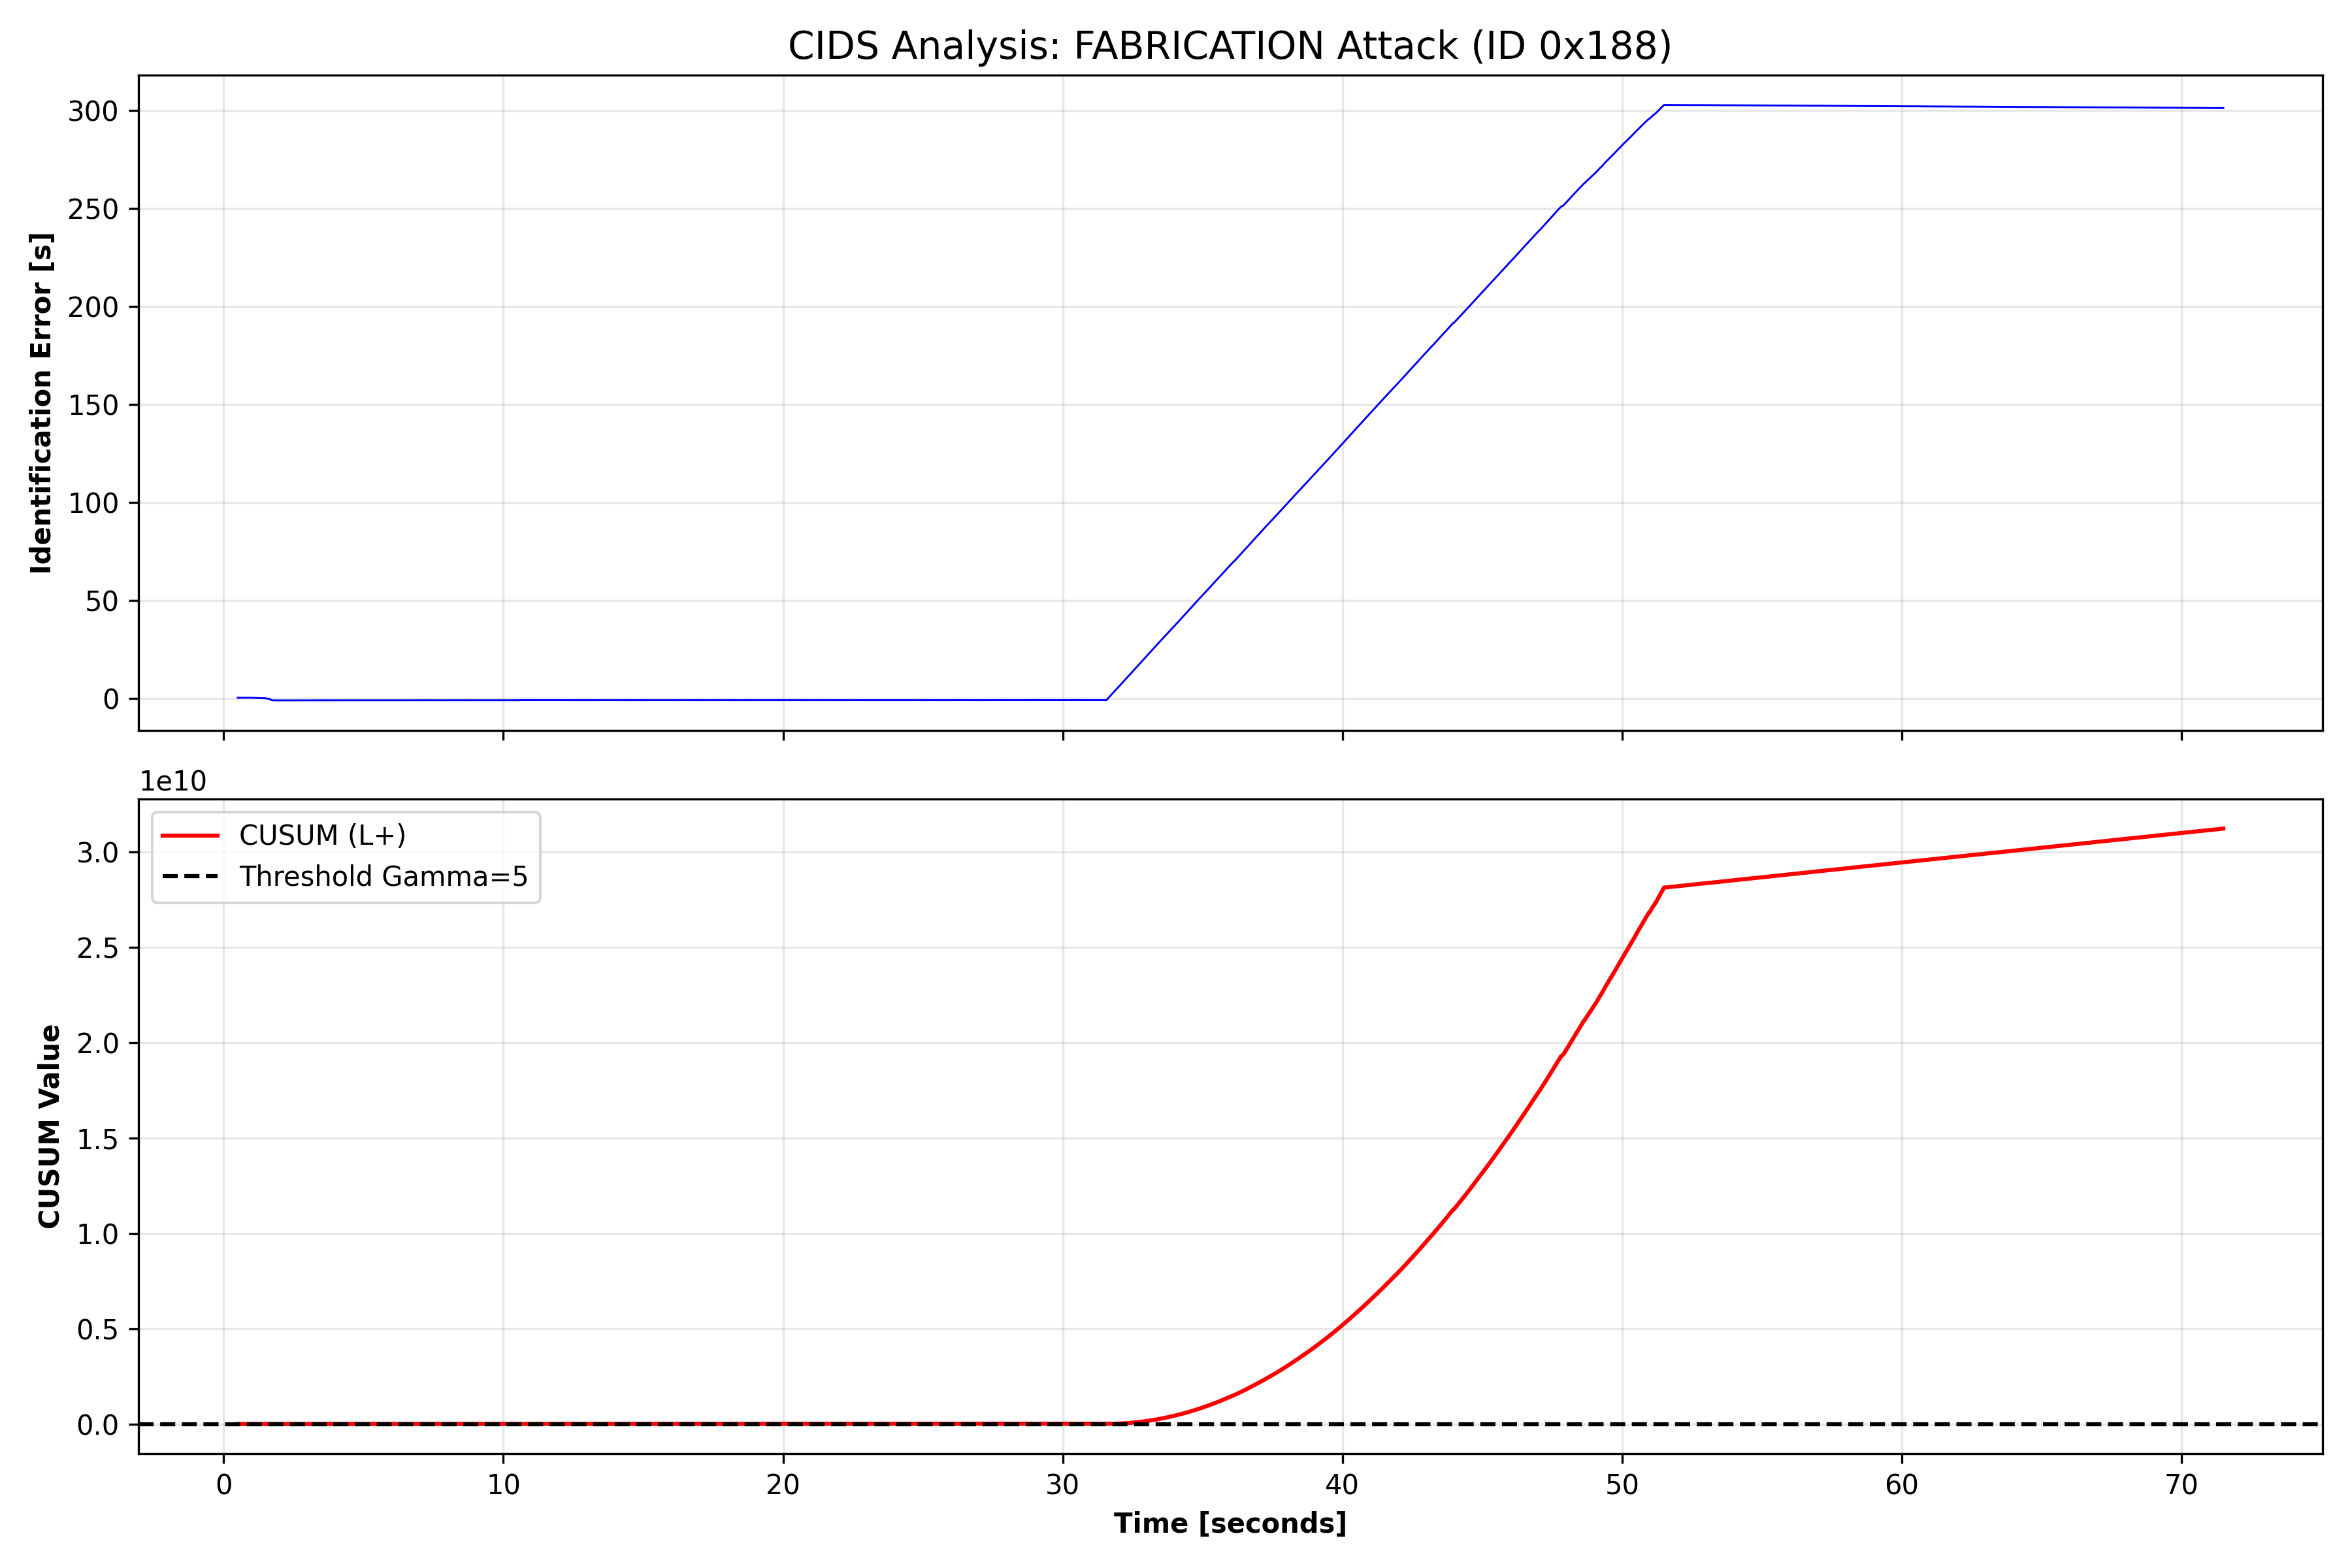
\includegraphics[width=0.95\textwidth]{../CIDS/cids_fabrication.png}
    \caption{CIDS Analysis: Fabrication Attack. Note the exponential explosion of the CUSUM value.}
    \label{fig:fabrication}
\end{figure*}

\vspace{1cm}

\begin{figure*}[h]
    \centering
    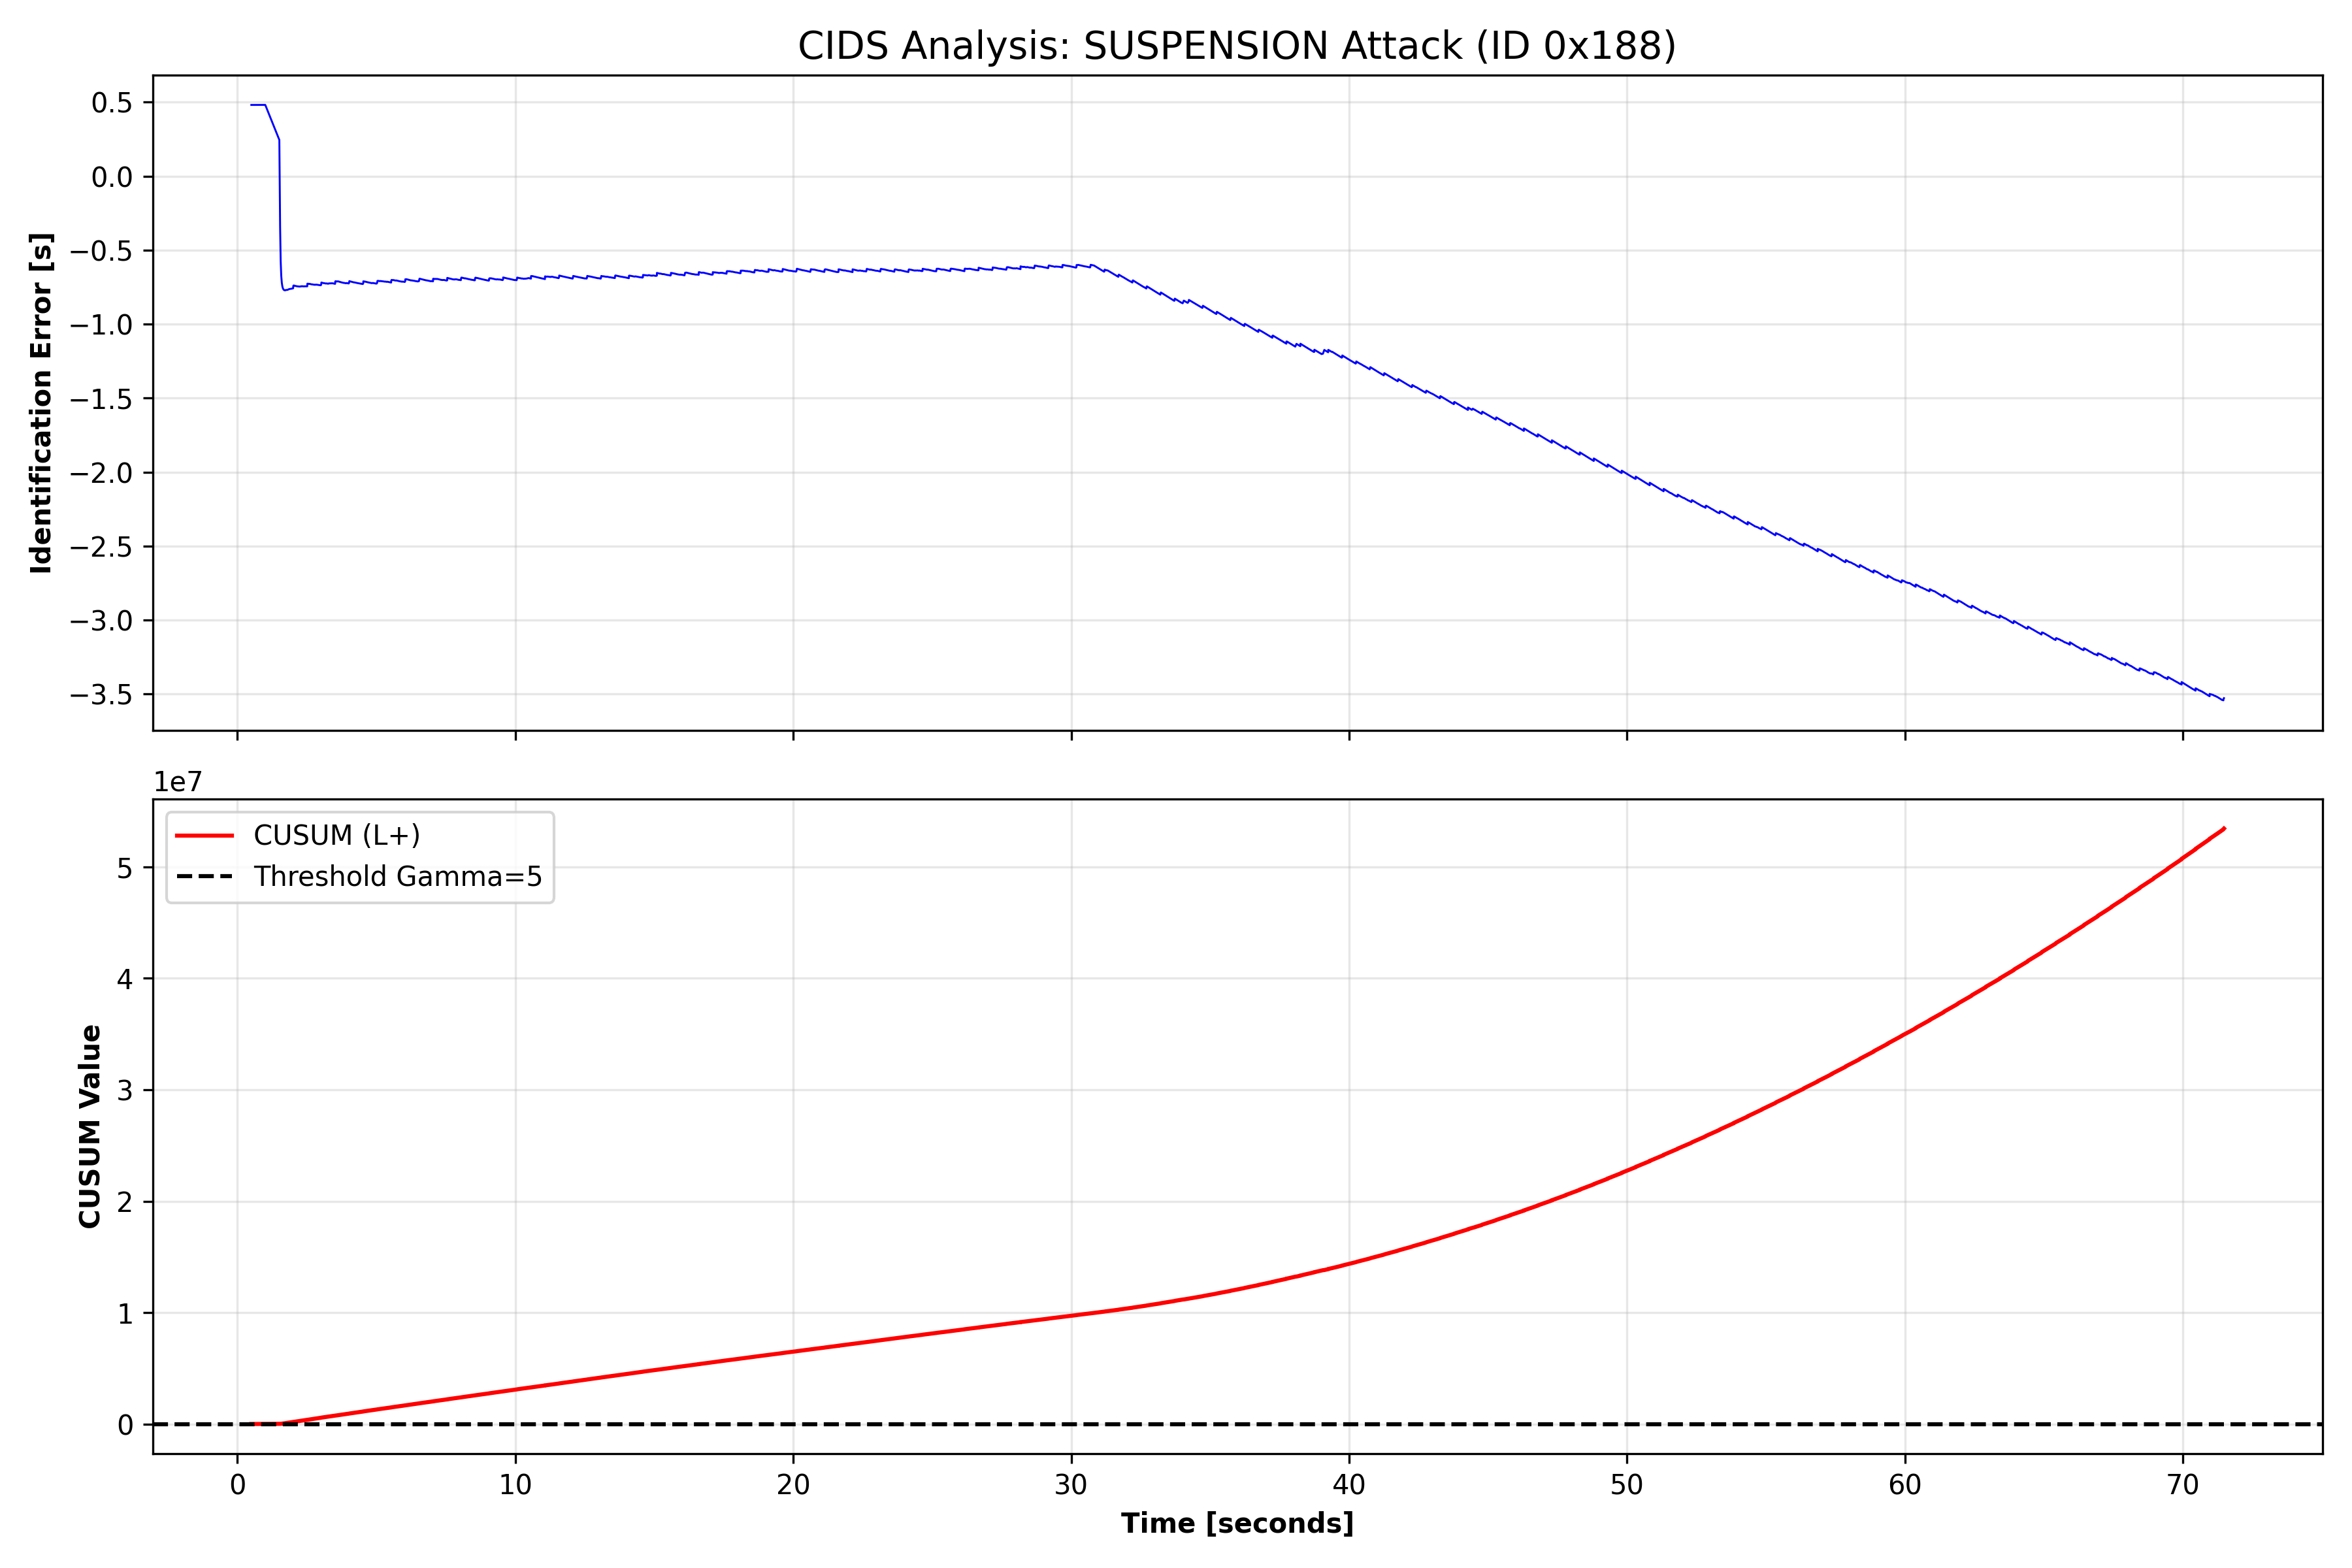
\includegraphics[width=0.95\textwidth]{../CIDS/cids_suspension.png}
    \caption{CIDS Analysis: Suspension Attack. Timing jitter caused by DoS results in logarithmic CUSUM growth.}
    \label{fig:suspension}
\end{figure*}

\vspace{1cm}

\begin{figure*}[h]
    \centering
    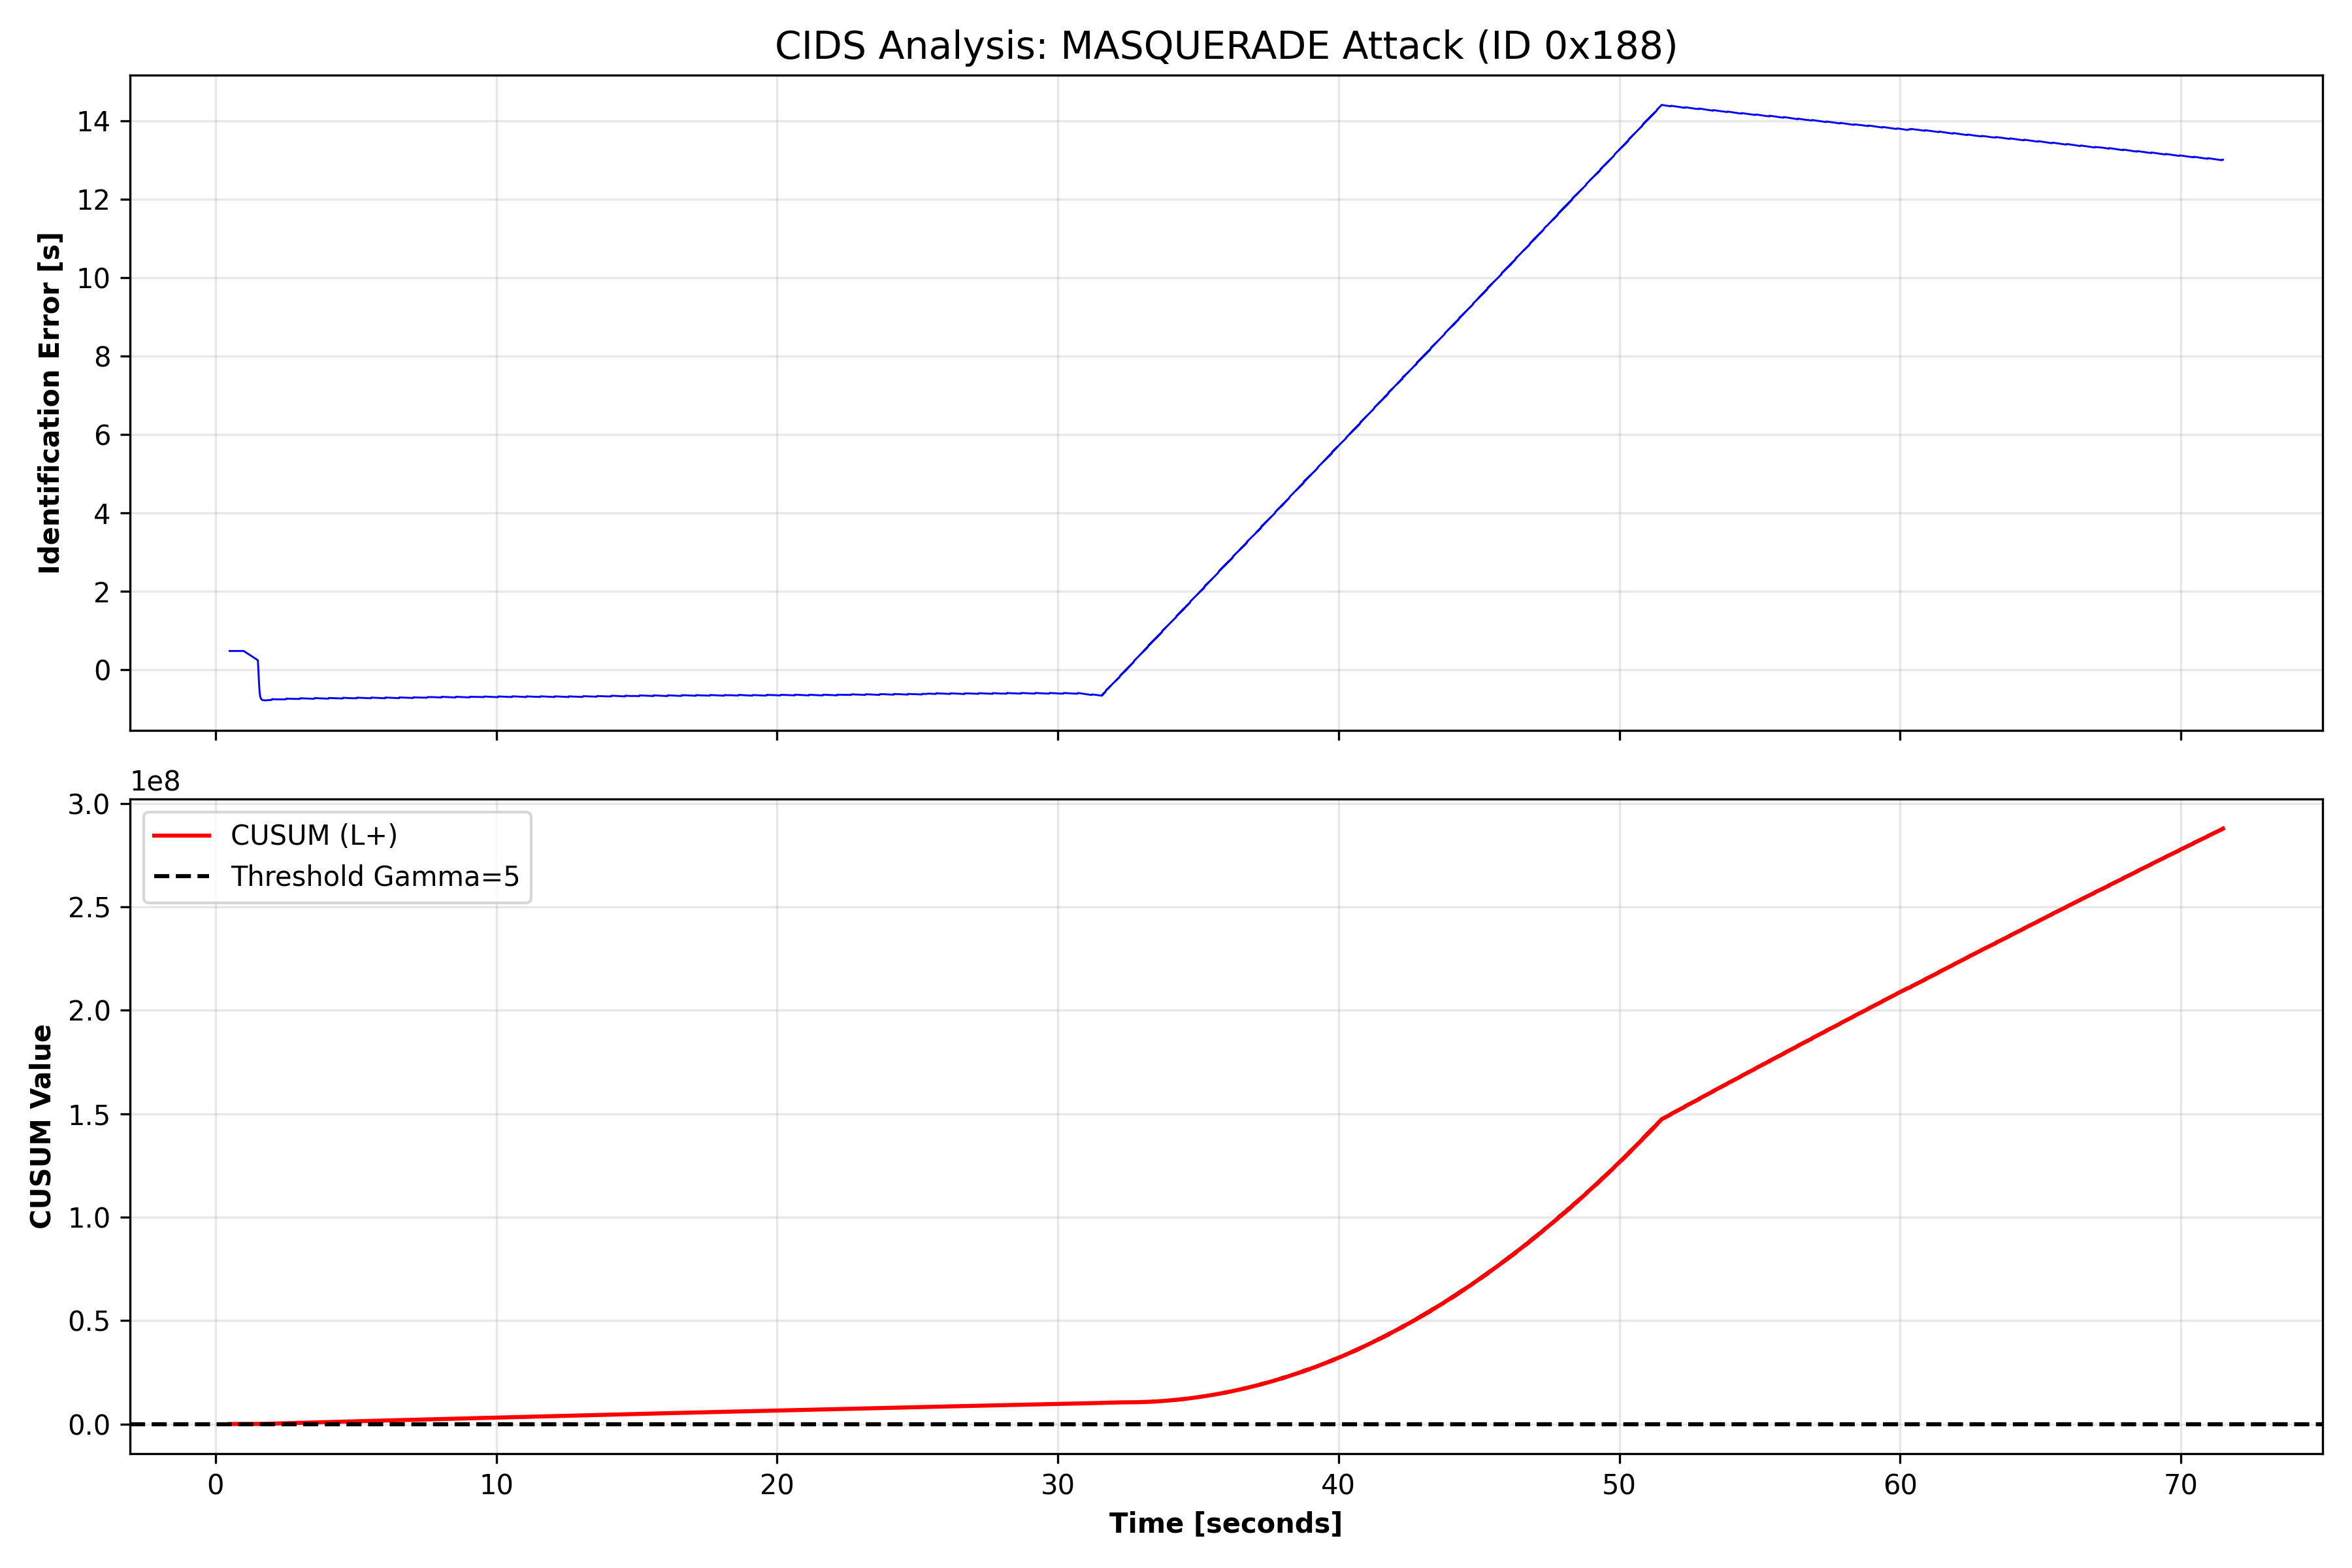
\includegraphics[width=0.95\textwidth]{../CIDS/cids_masquerade.png}
    \caption{CIDS Analysis: Masquerade Attack. The linear drift identifies the hardware clock discrepancy.}
    \label{fig:masquerade}
\end{figure*}

\end{document}